\section{目的}
依據 \textit{AIC Lab.pdf} 的 Chapter 1「Current Sinks and Sources」（PDF 實體頁碼 2--21），重寫並比較基本電流源、簡單電流鏡、cascode、高擺幅 cascode、Wilson、修正 Wilson、regulated 及 complete regulated 電流鏡。本次只交付 AIC Lab 1 預覽；原始程式作為尺寸與來源參考，講義的電路、問題與量測項目才是核對依據。

本報告採用由使用者另行提供的模型庫，供應電壓為 1.0 V。講義的 0.35 $\mu$m、3.3 V 模型、臨界電壓與數值圖表不能直接當作本次模型的驗收目標。1 V 是本次教學設計條件，並非對加密模型額定電壓的認證。

\section{Spec 對照}
所有頁碼皆為 PDF 的實體頁碼。表中「已模擬」表示具有真實 HSPICE 資料，不等同所有工作點都符合設計條件。5\% 比例誤差是本報告明訂的比較門檻，並非講義印出的保證規格。
\begin{longtable}{p{0.12\linewidth}p{0.38\linewidth}p{0.17\linewidth}p{0.22\linewidth}}
\toprule
頁碼/項目 & 核對要求 & 實作 deck & 狀態 \\
\midrule\endhead
2--4 / 1.1 & N/P I--V、輸出可用範圍、不同 $L$ 的輸出電阻 & 01 & 四種長度與閘極掃描已模擬 \\
5--7 / 1.2 & 50 $\mu$A；倍率 2/4/8/16；輸出 1/0.6/0.3/0.1 V & 02 & 原尺寸保留；低輸出電壓的失準已量出 \\
7 / 1.4 & 單位尺寸相同的原因、M0--M4 佈局 & 第六節 & 理論答覆；未宣稱完成 layout \\
8--10 / 2.1 & Cascode 複製電流、headroom、$R_o$ & 03 & 原條件超 rail；另列尺寸調整案例 \\
10--12 / 2.2、2.4 & 高擺幅、M4 尺寸、電流偏差原因 & 04、第六節 & 偏壓長度與電流變體已模擬 \\
13--16 / 3.1--3.3 & Wilson 與 modified Wilson 電流及電阻 & 05 & 相同工作點比較已完成 \\
17 / 3.4 & 交換 diode-connected 支路；比較 $R_o$ 階數 & 05、第六節 & 交換版本的失效案例保留 \\
18--19 / 4.1 & Regulated cascode 及額外偏壓支路 & 06 & 電流、偏壓、工作區已核對 \\
20 / 4.2 & Complete regulated cascode & 06 & 增補實作；case 4 通過本次工作點檢查 \\
21 / 4.4-Q1 & 完整比較表 & 第五節、CSV & 含電流誤差、$V_{min}$、$R_o$、功耗及 rail 裕量 \\
21 / 4.4-Q2 & 指定 $g_m^3/g_d^5$ 與其缺點 & 07、第六節 & 印刷式量綱不符；不宣稱完成字面目標 \\
\bottomrule
\end{longtable}

\section{電路與設計推導}
\subsection{基本關係與製程差異}
對同尺寸且相同偏壓的單位元件，理想電流鏡有
\[
\frac{I_o}{I_{ref}}\simeq\frac{(W/L)_o}{(W/L)_{ref}}=M,
\qquad r_o=\left(\frac{\partial I_D}{\partial V_{DS}}\right)^{-1}=\frac{1}{g_{ds}}.
\]
強反轉長通道近似給出 $V_{DS,min}\simeq V_{OV}$、$r_o\simeq1/(\lambda I_D)$；PMOS 應用 $V_{SD}$ 與 $V_{SG}$ 的正值大小判斷。Cascode 以局部負回授提高輸出電阻，近似 $R_o\simeq g_mr_o^2$；regulated 結構再加入增益，約為 $g_m^2r_o^3$。這些是趨勢公式，不能取代本次模型的操作點與導數。

講義的範例以 $\mu_n C_{ox}=166\,\mu\mathrm{A}/\mathrm{V}^2$、$V_T=0.55$ V、$W/L=3/1.4$、$I_{ref}=50\,\mu$A 算得 $V_{GS}\simeq1.08$ V、$V_{OV}\simeq0.53$ V；以 $\lambda=0.0209/\mathrm{V}$ 得 100/200 $\mu$A 支路約 478/239 k$\Omega$。這些是原講義的手算結果。本次量得 reference $V_{GS}=0.6591$ V，不能沿用上述參數或直接複製工作區結論。

\subsection{尺寸與案例的明確區分}
Deck 02--06 的 case 0 保留 $W_{unit}=3\,\mu$m、$L=1.4\,\mu$m、$I_{ref}=50\,\mu$A。Case 1 與 2 分別只改為 10 與 1 $\mu$A。Case 3 保持 50 $\mu$A 與 $L=1.4\,\mu$m，將單位寬度改為 30 $\mu$m，以降低電流密度與串疊所需 $V_{GS}$；這是另列的本次模型設計調整，不冒充原尺寸重現。

Deck 04 額外 case 4/5 在 1 $\mu$A、$W_{unit}=3\,\mu$m 下比較 M4 的 $L=3.5/14\,\mu$m（基準 7 $\mu$m）。Deck 06 的額外 case 4 採用 $W_{unit}=30\,\mu$m、MC2 寬度 120 $\mu$m、MC5/MC6 寬度 300 $\mu$m，其餘保持 case 3，以改善放大器負載的 headroom。新增完整 regulated 電路的 PMOS 尺寸屬本次設計，不是講義提供的數值。

\section{模擬設定}
七個獨立 \texttt{.sp} 均直接 include 指定模型，可由模擬器開啟；不依賴其他子電路檔。實際執行版本為 PrimeSim HSPICE S-2021.09 win64，溫度 27 $^\circ$C，共 30 個 base/alter 案例均完成，未出現 error 或 failed 量測。Deck 01 含四種長度，每種掃 11 個閘極電壓與 101 個汲極電壓。

輸出 DC 掃描 0--1 V、步進 1 mV；公平比較點固定 $V_o=0.8$ V。AC 以 1 V 擾動量得 1 Hz 的 $R_o=1/|I_{ac}|$。簡單鏡只有 VTEST 設為 AC=1，其餘固定輸出電壓源皆 AC=0；因此量的是單一輸出埠阻抗。以 0.799/0.801 V 的 DC 中央差分獨立核對。主要比較案例兩者差異小於 0.56\%，且 1 Hz 相位接近零；故此處將低頻阻抗大小近似為電阻。固定 M1--M4 支路表列的 $1/g_{ds}$ 是元件本身的小訊號電阻，與完整輸出埠量測的定義不同。

定義
\[
\epsilon_I=100\left(\frac{I_o}{2I_{ref}}-1\right)\%,\qquad
P_b=V_{DD}I_{bias,supply},\qquad P_o=V_oI_o.
\]
$V_{min,5\%}$ 是從該 1 mV 網格點起直到 1 V，所有後續點都滿足 $|\epsilon_I|\le5\%$ 且所列偏壓節點介於 0--1 V 的最小電壓。這是操作性定義，不等同理論的飽和邊界；未逐一認證整條掃描的元件工作區。表內 Check=Y 額外要求在 0.8 V 工作點，每顆相關 MOS 都有 $|V_{DS}|\ge|V_{DSAT}|$；保留 HSPICE 的 Subth 標籤，不把次臨界當成強反轉。

$P_b$ 只計偏壓電源支路；外接理想輸出電壓源另供應 $P_o$。兩者都不含實際參考電流產生器的設計成本。偏壓在 rail 內只是必要條件：理想 IREF 可以在極小裕量下供應指定電流，不能據此證明實體參考電流源可實現。

HSPICE 亦回報加密區塊的警告遭隱藏；以 \texttt{WARNLIMIT=100} 診斷仍無詳細訊息，因此不宣稱模擬為零警告。診斷量測與原結果一致，但不能據此判定警告無害。

\section{結果與規格檢查}
\subsection{元件長度與原始四支路例題}
在 $W=5\,\mu$m、$V_{GS}=V_{SG}=0.6$ V、$V_{DS}=V_{SD}=0.8$ V 下：

\begin{center}\small
\begin{tabular}{lrrrr}
\toprule
$L$ ($\mu$m) & $I_n$ ($\mu$A) & $|I_p|$ ($\mu$A) & $r_n$ (M$\Omega$) & $r_p$ (M$\Omega$) \\
\midrule
0.35 & 230.165 & 42.540 & 0.095 & 0.480 \\
0.70 & 110.800 & 19.204 & 0.300 & 1.718 \\
1.40 & 54.328 & 9.151 & 0.828 & 5.063 \\
2.80 & 26.860 & 4.465 & 2.231 & 14.243 \\
\bottomrule
\end{tabular}
\end{center}

較長 $L$ 的電阻提高，但同時電流也降低；因此本測試不是固定電流下單獨隔離 $\lambda$ 的實驗。

原尺寸 50 $\mu$A 例題的真實結果如下（電流來自零伏感測源，元件內部 $I_D$ 與端口電流可能因模型漏電略有差異）：

\begin{center}\small
\begin{tabular}{lrrrrrr}
\toprule
MOS & M & $V_{DS}$ (V) & $I_o$ ($\mu$A) & Error (\%) & Region & $1/g_{ds}$ (k$\Omega$) \\
\midrule
M1 & 2 & 1.0 & 99.971 & -0.029 & Saturation & 523.351 \\
M2 & 4 & 0.6 & 198.192 & -0.904 & Saturation & 186.878 \\
M3 & 8 & 0.3 & 388.246 & -2.939 & Saturation & 9.929 \\
M4 & 16 & 0.1 & 478.675 & -40.166 & Linear & 0.282 \\
\bottomrule
\end{tabular}
\end{center}

M3 在本次模型的此工作點仍被模型標為 Saturation，與舊講義的三極區判斷不同；M4 則為 Linear，不能期待得到理想 800 $\mu$A。這是實驗要觀察的低輸出電壓限制，不是把觀察到的失準隱藏成通過。

\subsection{原條件與本次模型的尺寸調整}
原尺寸 case 0，50 $\mu$A，$V_o=0.8$ V：

\begin{center}\small
\begin{tabular}{lrrrrr}
\toprule
Topology & $I_o$ ($\mu$A) & $\epsilon_I$ (\%) & $R_o$ (M$\Omega$) & $V_{b,max}$ (V) & Check \\
\midrule
Simple & 99.568 & -0.432 & 0.464 & 0.659 & Y \\
Cascode & 99.510 & -0.490 & 0.449 & 1.471 & N \\
High-swing & 99.958 & -0.042 & 10.021 & 1.092 & N \\
Wilson & 97.870 & -2.130 & 0.114 & 1.553 & N \\
Modified Wilson & 99.326 & -0.674 & 0.096 & 1.565 & N \\
Regulated & 99.771 & -0.229 & 0.442 & 1.560 & N \\
Complete regulated & 96.871 & -3.129 & 5.475 & 0.999 & N \\
\bottomrule
\end{tabular}
\end{center}

Case 0 的 cascode、high-swing、Wilson、modified Wilson、regulated 皆有偏壓超過 1 V；其曲線只是理想電流源支撐的數學解，不能視為 1 V 電路實作通過。Complete regulated 雖在 rail 內，仍有元件處於線性區。

調整為 $W_{unit}=30\,\mu$m 的 case 3，保持 50 $\mu$A：

\begin{center}\small
\begin{tabular}{lrrrrr}
\toprule
Topology & $I_o$ ($\mu$A) & $\epsilon_I$ (\%) & $R_o$ (M$\Omega$) & $V_{b,max}$ (V) & Check \\
\midrule
Simple & 100.770 & 0.770 & 0.324 & 0.440 & Y \\
Cascode & 99.781 & -0.219 & 10.175 & 0.975 & Y \\
High-swing & 100.063 & 0.063 & 3.724 & 0.571 & Y \\
Wilson & 98.143 & -1.857 & 10.353 & 0.973 & Y \\
Modified Wilson & 99.834 & -0.166 & 10.025 & 0.976 & Y \\
Regulated & 99.903 & -0.097 & 32.785 & 0.975 & Y \\
Complete regulated & 99.778 & -0.222 & 32.355 & 0.938 & N \\
\bottomrule
\end{tabular}
\end{center}

Complete regulated 的 case 3 仍未滿足全部元件工作區條件。追加 case 4 後，$I_o=99.5871\,\mu$A、誤差 $-0.4129\%$、$R_o=42.5508$ M$\Omega$、最高偏壓 0.8801 V，通過本次宣告的工作點檢查。MC2 的模型區域仍為 Subth，因此不能宣稱整個電路都在強反轉。

\begin{figure}[htbp]\centering
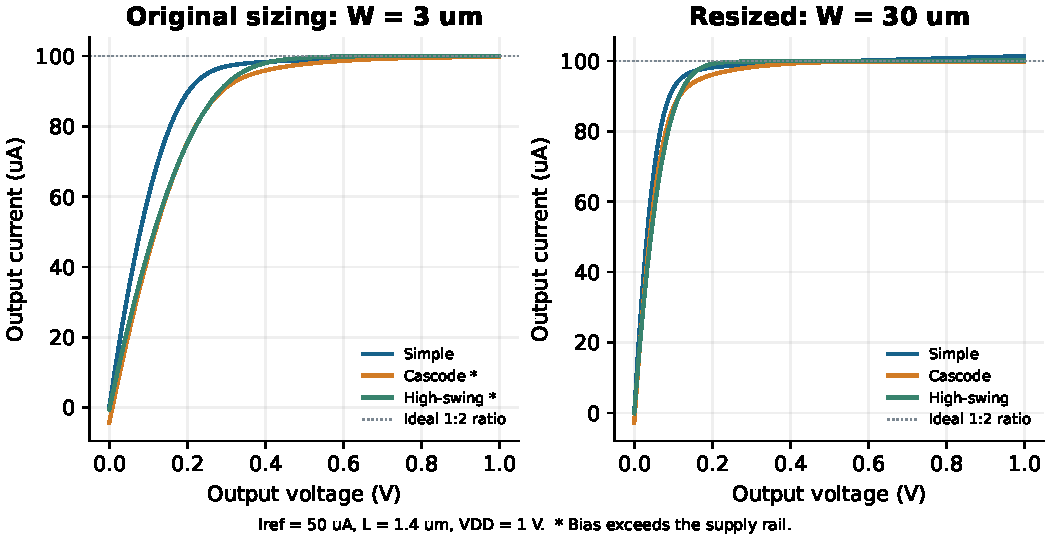
\includegraphics[width=\linewidth]{figures/aic01_mirrors.pdf}
\caption{真實 HSPICE DC 資料重繪的 simple/cascode/high-swing 比較；原尺寸與加寬尺寸皆為 50 $\mu$A。星號指出原條件的偏壓超 rail，該曲線不能當成 1 V 實體實作的通過證據。此圖不是 WaveView 截圖。}
\end{figure}

\begin{figure}[htbp]\centering
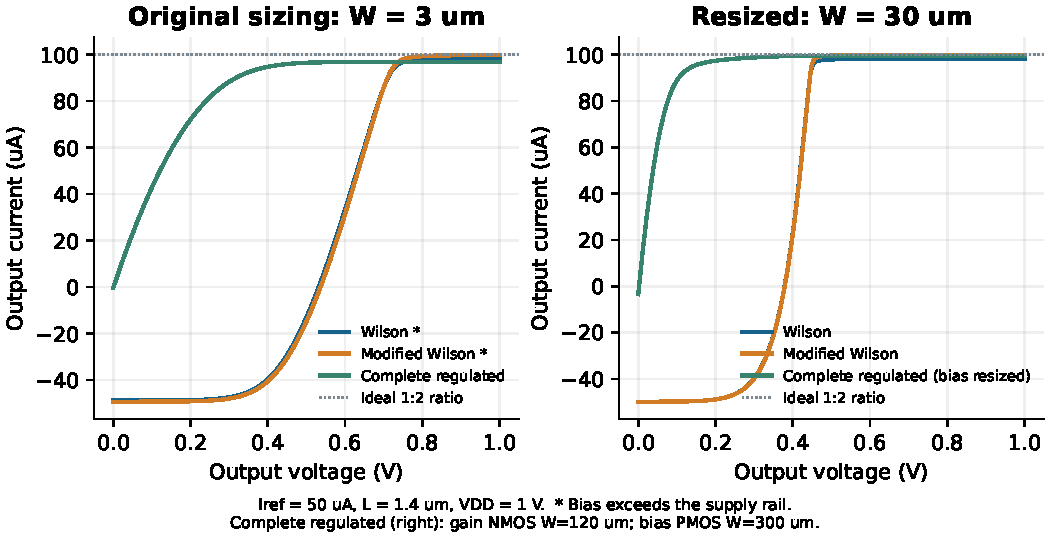
\includegraphics[width=\linewidth]{figures/aic01_feedback.pdf}
\caption{由真實 DC 資料重繪 Wilson、modified Wilson 與 complete regulated 曲線。Wilson/modified 的調整案例為 case 3；complete regulated 的最終偏壓尺寸調整為 case 4。原條件超 rail 的結果只作失效分析；圖形不是 WaveView 截圖。}
\end{figure}

操作範圍與功耗（case 3；完整 regulated 另列 case 4）：

\begin{center}\small
\begin{tabular}{lrrrrr}
\toprule
Topology & Case & $V_{min,5\%}$ (V) & $P_b$ ($\mu$W) & $P_o$ ($\mu$W) & Rail margin (V) \\
\midrule
Simple & 3 & 0.120 & 50.000 & 80.616 & 0.560 \\
Cascode & 3 & 0.173 & 50.000 & 79.825 & 0.025 \\
High-swing & 3 & 0.141 & 100.000 & 80.050 & 0.429 \\
Wilson & 3 & 0.496 & 50.000 & 78.514 & 0.027 \\
Modified Wilson & 3 & 0.500 & 50.000 & 79.867 & 0.024 \\
Regulated & 3 & 0.498 & 100.000 & 79.923 & 0.025 \\
Complete regulated & 3 & 0.142 & 130.021 & 79.823 & 0.062 \\
Complete regulated & 4 & 0.142 & 148.327 & 79.670 & 0.120 \\
\bottomrule
\end{tabular}
\end{center}

表中 $P_b$ 與 $P_o$ 是分開的功率項，不能把 $P_b$ 寫成總耗電。Cascode case 3 僅約 25 mV 的上電源裕量，尚未提供實際 IREF 元件所需的 compliance。空值表示宣告範圍內不存在符合定義的區間；不能用零取代。

\subsection{附加問題的量測}
交換 diode-connected 支路的版本，在加寬的 50 $\mu$A、0.8 V 案例得到 $I_o=18.1816\,\mu$A、參考節點約 2.809 V，未能在該工作點充當 1 V、1:2 電流鏡。這不是對所有可能偏壓的全域不可能性證明。

Deck 07 的有限頻寬理想回授放大器測試如下：

\begin{center}\small
\begin{tabular}{lrrr}
\toprule
A & $I_o$ ($\mu$A) & $R_o$ (M$\Omega$) & $V_g$ (V) \\
\midrule
1 & 57.975 & 2.415 & 0.705 \\
10 & 74.287 & 9.798 & 0.787 \\
100 & 78.141 & 51.695 & 0.809 \\
\bottomrule
\end{tabular}
\end{center}

增益提高可提高輸出阻抗，但此組固定 $V_{set}=0.15$ V 的支路並沒有達成 100 $\mu$A 複製電流；輸出阻抗大不代表電流比例正確。理想受控源不包含實際放大器耗電、輸出擺幅或 transistor 級穩定性設計。

\section{討論}
\begin{enumerate}
\item \textbf{相同單位尺寸與 layout（p7）}：相同 $W,L$ 可減少不同幾何造成的系統偏差，再以並聯單位數做倍率。1+2+4+8+16 共 31 單位，可讓 reference 單位位於中心，其餘以成對的對稱單位形成共同中心；使用相同方向、dummy 外圍與對稱低阻配線，並匹配接點與熱環境。這是佈局建議，沒有 GDS 或 mismatch 驗證。
\item \textbf{高擺幅 M4 尺寸與誤差（p12）}：忽略 body effect 時，希望 $V_{bias}\simeq V_T+2V_{OV}$；若 M4 與單位元件電流相同，強反轉平方律給 $(W/L)_4\simeq(W/L)_{unit}/4$。講義用長度 7 $\mu$m 作起點。實際還受 body effect、$V_{DS}$ 不匹配、短通道效應與漏電影響；04 的長度變體供比較。1 $\mu$A 案例可能為 Subth，不宜硬套平方律。對第 2.4-Q2 題，講義圖中高擺幅電流較小，應從不同內部 $V_{DS}$ 與偏壓、有限輸出電導及通道長度調變檢查；例如相同 $V_{GS}$ 時較低 $V_{DS}$ 可減少 CLM 帶來的電流增加。這不是拓樸必然的不等式，也不能只憑舊圖認定本模型必須同方向。本次模型 case 3 在相同 0.8 V 點，高擺幅為 100.063 $\mu$A、一般 cascode 為 99.781 $\mu$A，方向相反；保留真實觀察，不強湊舊結論。
\item \textbf{Wilson 交換 diode 與修改效果（p17）}：diode 的位置決定偏壓節點與回授路徑，不能只交換符號並假設仍具相同功能；第五節已保存失效案例。Modified Wilson 加入匹配 diode 以改善下方兩管的 $V_{DS}$ 對應；主導輸出電阻仍屬 $g_m r_o^2$ 階數。Case 3 的 Wilson/modified 分別約 10.353/10.025 M$\Omega$，電流誤差則由 $-1.857\%$ 改善至 $-0.166\%$，符合「精度改善而電阻階數相近」的觀察。
\item \textbf{Regulated 比較與功耗（p20、p21 Q1）}：增加回授增益可提高 $R_o$，但付出偏壓電流、面積、寄生極點與 headroom。完整版本也可能因負載管失去飽和而失效，所以不能只看輸出電流接近目標。講義 p20 另指出 M0/M1 的 $V_{DS}$ 不匹配仍會造成複製誤差；新增 M4--M6 不會自動消除此項。最終 case 4 的誤差仍為 $-0.413\%$，而非零。
\item \textbf{更高階輸出電阻（p21 Q2）}：$g_m$ 與 $g_d$ 單位都是 S，故 $g_m^3/g_d^5$ 的單位是 $\Omega^2$，不可能直接是一個電阻。若原意是再多一級無因次增益，可能要討論 $g_m^3/g_d^4$；此為推測，不能擅自當成講義正確目標。07 只驗證量綱正確的 $R_o\sim A g_mr_o^2$ 概念。要完成實際高階回授電流鏡，仍需確認題目、建立 transistor 放大器、檢查 loop gain/phase、啟動、雜訊、耗電與 PVT。字面規格保持未解決。
\end{enumerate}

\section{結論}
本次完成整章電路與問題的追蹤表、七個可執行 deck 及 30 個案例的真實 HSPICE 模擬；保留所有失準及超 rail 的證據。原尺寸不能直接在 1 V 下重現講義全部結果；另列的本次模型尺寸調整改善了比較工作點，完整 regulated 需額外偏壓尺寸調整。已通過的只有明訂的量測與操作點檢查，沒有宣稱完成實體 IREF、全 PVT、layout 或題目量綱疑義的驗收。

可追溯資料位於 \texttt{AIC/Lab01/results/}：各 case 的 CSV、量測數值匯出、\texttt{comparison.csv}、\texttt{operating\_points.csv} 與 \texttt{simulation\_data.json}。\texttt{manifest.json} 列出 spec 對照與案例定義。波形用來觀察整段行為；\texttt{.measure} 擷取有定義的量化指標，兩者一起核對。
